\section{Recommendation systems}\label{sec:recommendation-systems}

In Denmark when using apps to guide your travels, you will get choices as to the means of transport as in: by car,
train, bus, cycling or walking.
But if you wanted to prioritize your climate footprint you would have to research how much a specific means of
transportation pollutes.
Another situation is the economics of your travel.
Instead of having to calculate yourself how much money you would spend on a specific travel type, it could be done
automatically.
So to make it as easy as possible to make an informed decision, we want to automate many of these calculations, so the
users get an overview of their situation in a fast and easy way.

What we are really trying to do, is build a system that shows you the routes that you would want to travel based on your
personal preferences.
This can also be called a recommendation system (RS), this is something we all use every day, when browsing a web shop,
YouTube or other streaming services.
The goal of an RS is then to sort through all available data and present the most useful parts to the user.
As we can draw this parallel between our own project and something that already exists, we will now take a look at how
these systems are made.

A real world example of where this is used is in a movie recommender.
Movies are somewhat easy to classify, as one can look at the genres of different movies.
This type of RS works by filtering the movies through genres and is called content based filtering.
% TODO Reference figure in a more meaningful way.
See~\ref{fig:figure3} for more information.

\begin{figure}
    \centering
    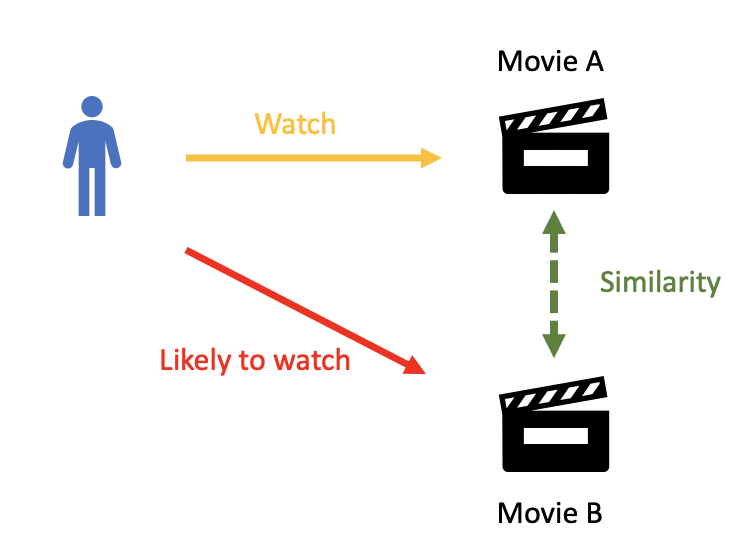
\includegraphics[width=\textwidth]{content-filtering}
    \caption{Content filtering.}
    \label{fig:figure3}
\end{figure}

An example would be user a watching an action movie, movie A, and the system would then remember user a's preferences
and recommend another action movie, movie B, to the user.\newline
This is a very simplified version of content filtering as they usually take multiple attributes from both the content
and the user.
In the context of a movie recommender this could be both the themes, the producer, the actors and so on.\newline
In content filtering, a user's history and interactions a used to create the profile for the RS to give suggestions.
Although content filtering is a lot better than giving random movies it does not take humans tendency to have changing
opinions and tastes.
Another type of filtering is Collaborative filtering (CB).
CB works by comparing users with each other.
This means that CB groups users by similarly watched movies, and then suggests movies from the users group.
% TODO Reference figure in a more meaningful way.
See~\ref{fig:figure4} for more information.

\begin{figure}
    \centering
    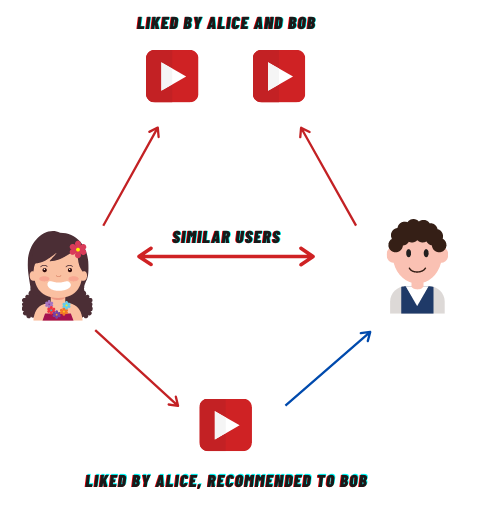
\includegraphics[width=\textwidth]{collaborative-filtering}
    \caption{Collaborative filtering.}
    \label{fig:figure4}
\end{figure}

By using CB you don't limit the recommendations to genres or other attributes that you already know the user watches it
can also recommend things from other genres, which would not have been recommended by the content filter.\newline
Generally for both these types of filters, they need a lot of information about both the user and the content, but that
is out of the scope of this project.
While content filters and collaborative filters are versatile in their use, our goal for this project is to use them to
recommend routes and make the user aware of both the monetary impact and the impact on our climate.
In this context, it would be more logical to get the users preferences directly through what could be a questionnaire,
rather than relying on behavior analysis.
The attributes one could use for the filters are straight forward, as they could be climate impact, cost, time and
others.
What would require some analysis would be getting useful data out of the routes we generate.
Using a weighted system to measure the results we get would allow us to choose the top \(1\,\%\) and by doing this we
have chosen the most relevant for the users.
